
\documentclass[11pt]{article}
\usepackage{fullpage}
\usepackage{graphicx}
\usepackage{pgfplots}
\graphicspath{ {images/} }

\title{\bf Targeted Layered Containment Studio}
\author{}
\date{}
\begin{document}
\maketitle

\section{Intervention Variables}
\label{int:var}
The kind of numerical data is very important 
\begin{itemize}
\item (Integer) type: 0 = vaccination, 1 = antiviral, 2 = social distancing, 3 = workClosure, 4 = schoolClosure, 5=infecting, 6=rollback, 7=stayHome
\item (Float) compliance: values from 0.0 to 1.0
\item (Int) duration: how many days this intervention action will be in effect
\item (Int) delay: period from the day when intervention is submitted to the day when it will become effective
\item (Float) efficacy-in: Node probability of getting infected by any other nodes, values from  0.0 to 1.0
\item  (Float) efficacy-out: Node probability of infecting other nodes, values from  0.0 to 1.0
\end{itemize}

\section{Ring Intervention} 
The trigger is the number of days before an infectious individual gets diagnosed, it will activate an intervention to every contact in his household. The intervention will be administrated to the household contacts if there's availability.

\subsection{Parameters to run the Ring intervention:}
The epistudy\_configs file has one intervention defined (intervention0)\\
\textbf{intervention0}
\begin{itemize}
\item iql\_key: key description of the intervention e.g: i0 (already defined for intervention0)
\item intervention variables (\ref{int:var})
\item (Float) ascertain: values from 0.0 to 1.0
\item (Int) days ill: days before an infectious individual gets diagnosed 
\item (Int) vaccines: number of vaccines
\item (Int) atday: beginning of the distribution
\end{itemize}

The README file inside the (epistudy\_configs/ring) folder has a detailed description of the intervention file.

\section{Household Intervention} 
\textbf{intervention0}: All symptomatic individuals retire home from the workplace after x days of being ill.\\
\textbf{intervention1}: Household contacts receive y days of treatment.

\subsection{Parameters to run the Household intervention:}
\textbf{intervention0}
\begin{itemize}
\item iql\_key: key description of the intervention e.g: i0 (already defined for intervention0)
\item intervention variables (\ref{int:var})
\item (Float) ascertain: values from 0.0 to 1.0
\item (Int) days ill: days before an infectious individual gets diagnosed 
\end{itemize}

\textbf{intervention1}
\begin{itemize}
\item iql\_key: key description of the intervention e.g: i1 (already defined for intervention1)
\item intervention variables (\ref{int:var})
\end{itemize}

The README file inside the (epistudy\_configs/household) folder has a detailed description of the intervention file.

\section{Isolation Intervention} 
\textbf{intervention0}: All symptomatic individuals retire home from the workplace after x days of being ill.\\
\textbf{intervention1}: Then isolate from contacts outside of home for x days.

\subsection{Parameters to run the Household intervention:}
\textbf{intervention0}
\begin{itemize}
\item iql\_key: key description of the intervention e.g: i0 (already defined for intervention0)
\item intervention variables (\ref{int:var})
\item (Float) ascertain: values from 0.0 to 1.0
\item (Int) days ill: days before an infectious individual gets diagnosed 
\end{itemize}

\textbf{intervention1}
\begin{itemize}
\item iql\_key: key description of the intervention e.g: i1 (already defined for intervention1)
\item intervention variables (\ref{int:var})
\end{itemize}

The README file inside the (epistudy\_configs/isolation) folder has a detailed description of the intervention file.

\section{Sweep}
\begin{itemize}
\item parameter: to sweep
\item (Float) start\_val: value starting the sweep
\item (Float) inc: value incrementing the value of the sweep
\item (Float) end\_val: value ending the sweep
\end{itemize}

e.g. Compliance values (0.5, 1.0):\\
$<start\_val>0.5</start\_val>\\
    <inc>0.5</inc>\\
    <end\_val>1.0</end\_val>$
    \\\\
e.g. Replicate values (0, 1):\\
$<start\_val>0</start\_val>\\
    <inc>1</inc>\\
    <end\_val>1</end\_val>$
    
\section{Epifast}
\begin{itemize}
\item seed: If it is desired that every time the simulation runs on the same configuration, it generates the same set of random realizations, then specify a fixed random seed in the xml configuration file as follows.
\end{itemize}
$<seed>7654321</seed>$\\
SimulationRandomSeed = 7654321
where $<seed>$ can be replaced by any integer.
If the value is not specified the default value for seed is 12345.

\section{Running the Intervention} 
To run the intervention: 
\begin{itemize}
\item Modify: epistudy\_cfg.xml
\item Run:
\begin{itemize}
\item $>$ . /home/pgxxc/public/dicex/dicex.sh
\item $>$ epistudy\_workflow.sh epistudy\_cfg.xml.
\end{itemize}
\end{itemize}

\section{Running the plots}
\begin{itemize}
\item Open the file dbsession\_Region\_Intervention.py to get the server\_ip value
\item Connect to the server\_ip e.g. ssh sfx058
\item Go to the study folder and run:
\begin{itemize}
\item $>$ . /home/pgxxc/public/dicex/dicex.sh
\item $>$ replicate\_analysis\_infections.sh epistudy\_cfg.xml
\end{itemize}
\end{itemize}

The following is an example of the household intervention infections plots running with compliance values of \{0,0.5,1.0\} for intervention 2, each with 2 replicates \{0,1\}.
 \begin{figure}[h]
\centering{\includegraphics[scale=0.5]{c_00_r_0infections_per_day.pdf}}
\caption{Compliance 0, Replicate 0}
\label{fig:indemics}
\end{figure}

 \begin{figure}[h]
\centering{\includegraphics[scale=0.5]{c_00_r_1infections_per_day.pdf}}
\caption{Compliance 0, Replicate 1}
\label{fig:indemics}
\end{figure}
 
  \begin{figure}[h]
\centering{\includegraphics[scale=0.5]{c_05_r_0infections_per_day.pdf}}
\caption{Compliance 0.5, Replicate 0}
\label{fig:indemics}
\end{figure}

 \begin{figure}[h]
\centering{\includegraphics[scale=0.5]{c_05_r_1infections_per_day.pdf}}
\caption{Compliance 0.5, Replicate 1}
\label{fig:indemics}
\end{figure}

 \begin{figure}[h]
\centering{\includegraphics[scale=0.5]{c_10_r_0infections_per_day.pdf}}
\caption{Compliance 1.0, Replicate 0}
\label{fig:indemics}
\end{figure}

 \begin{figure}[h]
\centering{\includegraphics[scale=0.5]{c_10_r_1infections_per_day.pdf}}
\caption{Compliance 1.0, Replicate 1}
\label{fig:indemics}
\end{figure}

 \begin{figure}[h]
\centering{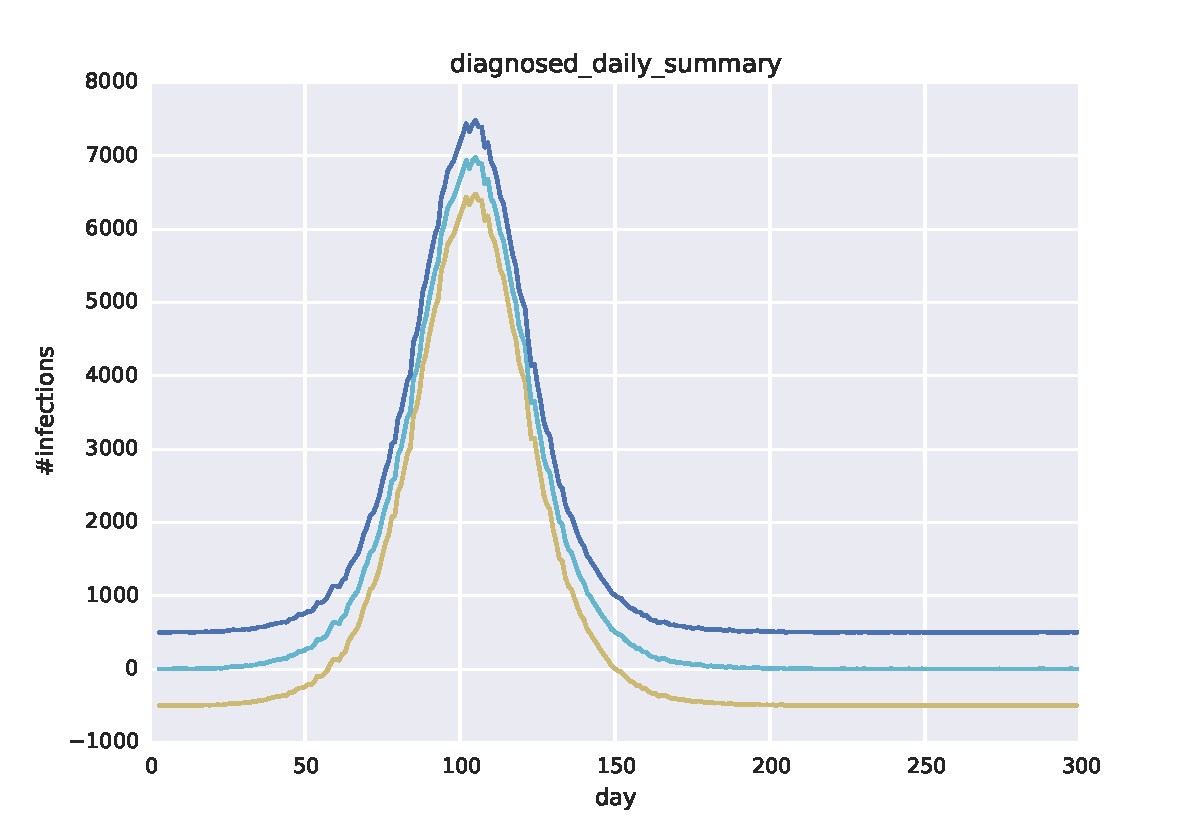
\includegraphics[scale=0.5]{diagnosed_daily_summary.pdf}}
\caption{Diagnosed Daily Summary}
\label{fig:indemics}
\end{figure}

\end{document}

